%==========================================================
%  PostgreSQL DVD Rental Practice Workbook
%  Author: Muhammad Usman
%  Colourful | Knowledge-Rich | Hint-Driven
%==========================================================
\documentclass[11pt,a4paper]{article}

%--- Core Layout ---
\usepackage[a4paper, top=2.2cm, bottom=2.2cm, left=2cm, right=2cm]{geometry}
\usepackage{parskip}

%--- Colour & Graphics ---
\usepackage[dvipsnames,svgnames,table]{xcolor}
\usepackage{tikz}
\usetikzlibrary{positioning,arrows.meta,shapes.geometric,backgrounds,fit,calc}
\usepackage{graphicx}

%--- Typography ---
\usepackage{pifont}\usepackage{marvosym}%\usepackage{lmodern}
\usepackage[T1]{fontenc}

%--- Code Listings ---
\usepackage{listings}
\usepackage{lstautogobble}

%--- Boxes & Frames ---
\usepackage[most]{tcolorbox}
\tcbuselibrary{breakable,skins,listings}

%--- Tables ---
\usepackage{booktabs}
\usepackage{tabularx}
\usepackage{array}
\usepackage{multirow}

%--- Misc ---
\usepackage{enumitem}
\usepackage{hyperref}
\usepackage{titlesec}
\usepackage{fancyhdr}
\usepackage{mdframed}
\usepackage{etoolbox}
\usepackage{adjustbox}
\usepackage{needspace}

%==========================================================
%  COLOUR PALETTE
%==========================================================
\definecolor{PgBlue}     {RGB}{51,  103, 145}   % PostgreSQL elephant blue
\definecolor{PgDark}     {RGB}{24,  60,  90}    % dark navy
\definecolor{PgLight}    {RGB}{210, 230, 245}   % pale blue
\definecolor{AccentGold} {RGB}{220, 160, 30}    % gold accent
\definecolor{AccentRed}  {RGB}{196, 58,  58}    % warm red
\definecolor{AccentGreen}{RGB}{56,  140, 80}    % green
\definecolor{AccentPurple}{RGB}{100, 65, 160}   % purple
\definecolor{AccentOrange}{RGB}{210, 105, 30}   % orange
\definecolor{HintBg}     {RGB}{255, 250, 235}   % warm ivory
\definecolor{TipBg}      {RGB}{236, 250, 240}   % soft green bg
\definecolor{WarnBg}     {RGB}{255, 240, 240}   % soft red bg
\definecolor{ConceptBg}  {RGB}{240, 240, 255}   % lavender bg
\definecolor{CodeBg}     {RGB}{28,  35,  46}    % dark code bg
\definecolor{CodeFg}     {RGB}{220, 225, 235}   % code fg
\definecolor{KeywordClr} {RGB}{130, 200, 255}   % SQL keyword
\definecolor{StringClr}  {RGB}{195, 232, 141}   % string
\definecolor{CommentClr} {RGB}{130, 148, 150}   % comment
\definecolor{NumberClr}  {RGB}{255, 180, 90}    % number
\definecolor{FuncClr}    {RGB}{255, 200, 120}   % function
\definecolor{LightGray}  {RGB}{248, 248, 248}
\definecolor{MidGray}    {RGB}{180, 180, 180}

%==========================================================
%  LISTINGS CONFIG
%==========================================================
\lstdefinestyle{sqlstyle}{
  language=SQL,
  backgroundcolor=\color{CodeBg},
  basicstyle=\ttfamily\small\color{CodeFg},
  keywordstyle=\color{KeywordClr}\bfseries,
  keywordstyle=[2]\color{FuncClr},
  stringstyle=\color{StringClr},
  commentstyle=\color{CommentClr}\itshape,
  numberstyle=\color{NumberClr},
  breaklines=true,
  showstringspaces=false,
  tabsize=2,
  autogobble=true,
  frame=none,
  xleftmargin=6pt,
  xrightmargin=6pt,
  aboveskip=0pt,
  belowskip=0pt,
  morekeywords={RETURNING,SERIAL,BIGSERIAL,BOOLEAN,EXPLAIN,ANALYZE,VACUUM,
    MATERIALIZED,REFRESH,LATERAL,PARTITION,RANGE,BRIN,GIN,GIST,
    TABLESPACE,CONCURRENTLY,PREPARE,EXECUTE,DEALLOCATE,
    TSVECTOR,TSQUERY,PLAINTO_TSQUERY,ILIKE,SIMILAR,ROLLUP,CUBE,
    GROUPING,SETS,FILTER,WITHIN,OVER,PRECEDING,FOLLOWING,
    UNBOUNDED,CURRENT,ROW,ROWS,RANGE,GROUPS,EXCLUDE,TIES,
    RAISE,NOTICE,EXCEPTION,LANGUAGE,PLPGSQL,BEGIN,END,
    IF,THEN,ELSIF,ELSE,LOOP,WHILE,FOR,RETURN,RETURNS,
    DECLARE,RECORD,ALIAS,PERFORM,FOUND,OLD,NEW,
    CASCADE,RESTRICT,DEFERRABLE,DEFERRED,IMMEDIATE,
    INHERITS,LIKE,INCLUDING,EXCLUDING,DEFAULTS,CONSTRAINTS},
  morekeywords=[2]{COUNT,SUM,AVG,MIN,MAX,COALESCE,NULLIF,GREATEST,LEAST,
    ROW_NUMBER,RANK,DENSE_RANK,LEAD,LAG,FIRST_VALUE,LAST_VALUE,
    NTH_VALUE,PERCENT_RANK,CUME_DIST,NTILE,
    DATE_TRUNC,DATE_PART,EXTRACT,NOW,CURRENT_DATE,CURRENT_TIMESTAMP,
    INTERVAL,AGE,TO_CHAR,TO_DATE,TO_TIMESTAMP,
    LENGTH,UPPER,LOWER,TRIM,LTRIM,RTRIM,SUBSTRING,REPLACE,
    CONCAT,SPLIT_PART,REGEXP_REPLACE,REGEXP_MATCH,
    ARRAY_AGG,STRING_AGG,JSON_AGG,JSONB_AGG,
    UNNEST,GENERATE_SERIES,PG_TYPEOF,PG_STAT_STATEMENTS}
}
\lstset{style=sqlstyle}

%==========================================================
%  TCOLORBOX ENVIRONMENTS
%==========================================================

% -- Code block with dark background --
\tcbuselibrary{listings}
\newtcblisting{sqlcode}[1][]{
  colback=CodeBg, colframe=PgBlue!60, colupper=CodeFg,
  listing only,
  listing options={style=sqlstyle},
  fonttitle=\bfseries\small\color{white},
  title={\texttt{</>}\quad SQL},
  arc=4pt, boxrule=0.6pt,
  left=6pt, right=6pt, top=4pt, bottom=4pt,
  breakable,
  #1
}

% -- Concept box (lavender) --
\newtcolorbox{conceptbox}[1]{
  colback=ConceptBg, colframe=AccentPurple!70,
  fonttitle=\bfseries\color{AccentPurple},
  title={\ding{72}\quad Concept: #1},
  arc=5pt, boxrule=0.7pt,
  left=8pt, right=8pt, top=6pt, bottom=6pt,
  breakable
}

% -- Hint box (warm ivory) --
\newtcolorbox{hintbox}{
  colback=HintBg, colframe=AccentGold!80,
  fonttitle=\bfseries\color{AccentGold!80!black},
  title={\ding{72}\quad Hint},
  arc=5pt, boxrule=0.7pt,
  left=8pt, right=8pt, top=6pt, bottom=6pt,
  breakable
}

% -- Tip box (green) --
\newtcolorbox{tipbox}{
  colback=TipBg, colframe=AccentGreen!70,
  fonttitle=\bfseries\color{AccentGreen!80!black},
  title={\ding{52}\quad Pro Tip},
  arc=5pt, boxrule=0.7pt,
  left=8pt, right=8pt, top=6pt, bottom=6pt,
  breakable
}

% -- Warning box (red) --
\newtcolorbox{warnbox}{
  colback=WarnBg, colframe=AccentRed!70,
  fonttitle=\bfseries\color{AccentRed},
  title={\textbf{(!)}\quad Watch Out},
  arc=5pt, boxrule=0.7pt,
  left=8pt, right=8pt, top=6pt, bottom=6pt,
  breakable
}

% -- Schema box --
\newtcolorbox{schemabox}{
  colback=PgLight!60, colframe=PgBlue!60,
  fonttitle=\bfseries\color{PgDark},
  title={\textbf{[DB]}\quad Schema Quick Reference},
  arc=5pt, boxrule=0.7pt,
  left=8pt, right=8pt, top=6pt, bottom=6pt,
  breakable
}

% -- Key concept summary box --
\newtcolorbox{keybox}[1]{
  colback=PgDark!8, colframe=PgDark!40,
  fonttitle=\bfseries\color{PgDark},
  title={#1},
  arc=5pt, boxrule=0.7pt,
  left=8pt, right=8pt, top=6pt, bottom=6pt,
  breakable
}

% -- Section header box --
\newtcolorbox{sectionheader}[2]{
  colback=#1, colframe=#1!80!black,
  fontupper=\bfseries\large\color{white},
  arc=6pt, boxrule=0pt,
  left=10pt, right=10pt, top=8pt, bottom=8pt,
  before upper={\S\quad},
  title={},
  #2
}

%==========================================================
%  DIFFICULTY BADGES
%==========================================================
\newcommand{\easy}{%
  
\begin{tikzpicture}[baseline=-1mm]
    \node[fill=AccentGreen!25, draw=AccentGreen!70, rounded corners=3pt,
          inner xsep=5pt, inner ysep=2pt,
          font=\tiny\bfseries\color{AccentGreen!80!black}] {\ding{109}\,EASY};
  \end{tikzpicture}}

\newcommand{\medium}{%
  
\begin{tikzpicture}[baseline=-1mm]
    \node[fill=AccentGold!25, draw=AccentGold!70, rounded corners=3pt,
          inner xsep=5pt, inner ysep=2pt,
          font=\tiny\bfseries\color{AccentGold!80!black}] {\ding{108}\,MEDIUM};
  \end{tikzpicture}}

\newcommand{\hard}{%
  
\begin{tikzpicture}[baseline=-1mm]
    \node[fill=AccentRed!20, draw=AccentRed!60, rounded corners=3pt,
          inner xsep=5pt, inner ysep=2pt,
          font=\tiny\bfseries\color{AccentRed}] {\ding{115}\,HARD};
  \end{tikzpicture}}

\newcommand{\expert}{%
  
\begin{tikzpicture}[baseline=-1mm]
    \node[fill=AccentPurple!20, draw=AccentPurple!60, rounded corners=3pt,
          inner xsep=5pt, inner ysep=2pt,
          font=\tiny\bfseries\color{AccentPurple}] {\ding{72}\,EXPERT};
  \end{tikzpicture}}

%==========================================================
%  SECTION HEADING STYLE
%==========================================================
\titleformat{\section}
  {\normalfont\Large\bfseries\color{PgDark}}
  {\thesection}
  {0.5em}
  {\colorbox{PgBlue!90}{\parbox{\dimexpr\textwidth-2\fboxsep-1em\relax}{\textcolor{white}{##1}}}}

\titleformat{\subsection}
  {\normalfont\normalsize\bfseries\color{PgDark}}
  {\thesubsection}
  {0.5em}
  {}
  [\vspace{-4pt}\textcolor{PgBlue!50}{\rule{\linewidth}{0.5pt}}]

%==========================================================
%  HEADER / FOOTER
%==========================================================
\pagestyle{fancy}
\fancyhf{}
\fancyhead[L]{\small\color{PgDark}\textbf{PostgreSQL Workbook} \textcolor{MidGray}{|} DVD Rental}
\fancyhead[R]{\small\color{PgDark}Muhammad Usman}
\fancyfoot[C]{\small\color{MidGray}\thepage}
\fancyfoot[R]{\small\color{MidGray}\textbf{[DB]}\ dvdrental}
\renewcommand{\headrulewidth}{0.4pt}
\renewcommand{\headrule}{\hbox to\headwidth{\color{PgBlue}\leaders\hrule height \headrulewidth\hfill}}

%==========================================================
%  HYPERREF
%==========================================================
\hypersetup{
  colorlinks=true,
  linkcolor=PgBlue,
  urlcolor=AccentGreen!70!black,
  citecolor=AccentPurple
}

%==========================================================
%  CUSTOM LIST STYLE
%==========================================================
\setlist[enumerate,1]{
  label=\textcolor{PgBlue}{\textbf{\arabic*.}},
  leftmargin=1.6em,
  itemsep=6pt
}

%==========================================================
%  HELPER: question item with badge
%==========================================================
\newcommand{\qitem}[2]{\item #1 \hfill #2}

%==========================================================
%  DOCUMENT BEGIN
%==========================================================
\begin{document}

%----------------------------------------------------------
%  COVER PAGE
%----------------------------------------------------------
\begin{titlepage}
\pagecolor{PgDark}
\begin{tikzpicture}[remember picture, overlay]
  % Background grid
  \foreach \x in {0,1,...,40}
    \draw[PgBlue!30, very thin] (\x*0.6-5, -25) -- (\x*0.6-5, 5);
  \foreach \y in {0,1,...,40}
    \draw[PgBlue!30, very thin] (-5, \y*0.6-25) -- (25, \y*0.6-25);
  % Big elephant motif (abstract circles)
  \fill[PgBlue!25] (16,-10) circle (5.5cm);
  \fill[PgBlue!15] (16,-10) circle (4.0cm);
  \draw[PgBlue!50, thick] (16,-10) circle (5.5cm);
\end{tikzpicture}

\vspace*{3cm}
\begin{center}
  {\fontsize{11}{13}\selectfont\color{AccentGold}\textbf{\textbf{[DB]}\quad POSTGRESQL PRACTICE WORKBOOK}}\\[1em]
  {\fontsize{32}{36}\selectfont\color{white}\textbf{DVD Rental}}\\[0.3em]
  {\fontsize{32}{36}\selectfont\color{PgBlue!60!white}\textbf{Database}}\\[0.5em]
  {\fontsize{14}{17}\selectfont\color{PgLight!80} Basic $\longrightarrow$ Advanced}\\[3em]

  
\begin{tikzpicture}
    \draw[AccentGold, line width=1.5pt] (-5,0) -- (5,0);
  \end{tikzpicture}\\[2em]

  {\large\color{white} \textbf{Muhammad Usman}}\\[0.4em]
  {\normalsize\color{MidGray} Data Engineering \& Cloud Architecture}\\[3em]

  \begin{tcolorbox}[
    width=0.72\linewidth,
    colback=PgBlue!30!PgDark,
    colframe=AccentGold!60,
    arc=8pt, boxrule=0.8pt,
    halign=center
  ]
  \color{PgLight}\small
  \textbf{21 Topics}\enspace\textcolor{AccentGold}{$\bullet$}\enspace
  \textbf{105 Questions}\enspace\textcolor{AccentGold}{$\bullet$}\enspace
  \textbf{SQL Hints \& Answers}\enspace\textcolor{AccentGold}{$\bullet$}\enspace
  \textbf{Concept Guides}
  \end{tcolorbox}
\end{center}
\vfill
\begin{center}
  \color{MidGray}\small Compiled for the \texttt{dvdrental} PostgreSQL sample database
\end{center}
\end{titlepage}
\nopagecolor

%----------------------------------------------------------
%  SCHEMA OVERVIEW PAGE
%----------------------------------------------------------
\newpage
\thispagestyle{fancy}

\begin{center}
{\Large\bfseries\color{PgDark}\textbf{[DB]}\quad DVD Rental --- Entity Relationship Diagram}
\end{center}
\vspace{0.3em}

\tikzset{
  ent/.style={
    draw=PgBlue, fill=PgLight!70, rounded corners=5pt,
    minimum width=2.4cm, minimum height=0.65cm,
    font=\small\bfseries\color{PgDark}, align=center, thick
  },
  junc/.style={
    draw=AccentPurple!70, fill=AccentPurple!12, rounded corners=5pt,
    minimum width=2.4cm, minimum height=0.65cm,
    font=\small\bfseries\color{AccentPurple}, align=center
  },
  tx/.style={
    draw=AccentGold!80, fill=AccentGold!10, rounded corners=5pt,
    minimum width=2.4cm, minimum height=0.65cm,
    font=\small\bfseries\color{AccentGold!80!black}, align=center
  },
  geo/.style={
    draw=AccentGreen!70, fill=AccentGreen!12, rounded corners=5pt,
    minimum width=2.4cm, minimum height=0.65cm,
    font=\small\bfseries\color{AccentGreen!70!black}, align=center
  },
  arr/.style={-{Stealth[length=5pt]}, thick, color=PgBlue!60},
  lbl/.style={font=\tiny\color{AccentRed}\bfseries, midway}
}

\begin{center}
\begin{tikzpicture}[node distance=1.8cm and 2.0cm]

% Geography cluster
\node[geo] (country) {COUNTRY};
\node[geo, right=of country] (city) {CITY};
\node[geo, right=of city] (address) {ADDRESS};

% People
\node[ent, right=of address] (customer) {CUSTOMER};
\node[ent, below=1.4cm of address] (store) {STORE};
\node[ent, below=1.4cm of customer] (staff) {STAFF};

% Film cluster
\node[ent, below=1.4cm of city] (film) {FILM};
\node[ent, left=of film] (language) {LANGUAGE};
\node[junc, left=1.6cm of language] (actor) {ACTOR};

% Junctions
\node[junc, below=1.4cm of actor] (filmactor) {FILM\_ACTOR};
\node[junc, below=1.4cm of film] (filmcat) {FILM\_CATEGORY};
\node[junc, right=1.6cm of film] (category) {CATEGORY};

% Operational
\node[tx, below=1.4cm of store] (inventory) {INVENTORY};
\node[tx, below=1.4cm of inventory] (rental) {RENTAL};
\node[tx, right=of rental] (payment) {PAYMENT};

% Geography arrows
\draw[arr] (country) -- node[lbl,above]{1:N} (city);
\draw[arr] (city)    -- node[lbl,above]{1:N} (address);
\draw[arr] (address) -- node[lbl,above]{1:N} (customer);
\draw[arr] (address) -- node[lbl,right]{1:N} (store);
\draw[arr] (address) -- node[lbl,right]{1:N} (staff);

% Store / Staff
\draw[arr] (store)    -- node[lbl,right]{1:N} (customer);
\draw[arr] (store)    -- node[lbl,left]{1:N}  (staff);
\draw[arr] (store)    -- node[lbl,right]{1:N} (inventory);

% Film
\draw[arr] (language) -- node[lbl,above]{1:N} (film);
\draw[arr] (film)     -- node[lbl,right]{1:N} (inventory);
\draw[arr] (film)     -- node[lbl,right]{M:N} (filmcat);
\draw[arr] (film)     -- node[lbl,left] {M:N} (filmactor);
\draw[arr] (actor)    -- node[lbl,left] {M:N} (filmactor);
\draw[arr] (category) -- node[lbl,right]{M:N} (filmcat);

% Operational
\draw[arr] (inventory) -- node[lbl,right]{1:N} (rental);
\draw[arr] (customer)  -- node[lbl,right]{1:N} (rental);
\draw[arr] (staff)     -- node[lbl,right]{1:N} (rental);
\draw[arr] (rental)    -- node[lbl,above]{1:N} (payment);
\draw[arr] (customer)  -- node[lbl,above]{1:N} (payment);
\draw[arr] (staff)     -- node[lbl,right]{1:N} (payment);

\end{tikzpicture}
\end{center}

\vspace{0.5em}
\begin{center}
\begin{tikzpicture}
  \node[geo, minimum width=1.5cm] (g1) {Geography};
  \node[ent, right=0.4cm of g1, minimum width=1.5cm] (g2) {Core Entity};
  \node[junc, right=0.4cm of g2, minimum width=1.5cm] (g3) {Junction};
  \node[tx, right=0.4cm of g3, minimum width=1.5cm] (g4) {Transactional};
\end{tikzpicture}
\end{center}

\vspace{0.8em}
\begin{schemabox}
\small
\begin{tabularx}{\linewidth}{@{} l X @{}}
\toprule
\textbf{Table} & \textbf{Key Columns} \\
\midrule
\texttt{film}       & film\_id PK, title, description, release\_year, language\_id FK, rental\_duration, \textbf{rental\_rate}, length, replacement\_cost, \textbf{rating}, fulltext (tsvector) \\
\texttt{actor}      & actor\_id PK, first\_name, last\_name \\
\texttt{category}   & category\_id PK, name \\
\texttt{language}   & language\_id PK, name \\
\texttt{inventory}  & inventory\_id PK, film\_id FK, \textbf{store\_id} FK \\
\texttt{rental}     & rental\_id PK, rental\_date, inventory\_id FK, customer\_id FK, \textbf{return\_date}, staff\_id FK \\
\texttt{payment}    & payment\_id PK, customer\_id FK, staff\_id FK, rental\_id FK, \textbf{amount}, payment\_date \\
\texttt{customer}   & customer\_id PK, store\_id FK, first\_name, last\_name, \textbf{email}, address\_id FK, \textbf{active} \\
\texttt{staff}      & staff\_id PK, first\_name, last\_name, store\_id FK, email, active \\
\texttt{store}      & store\_id PK, \textbf{manager\_staff\_id} FK, address\_id FK \\
\texttt{address}    & address\_id PK, address, city\_id FK, postal\_code \\
\texttt{city}       & city\_id PK, city, country\_id FK \\
\texttt{country}    & country\_id PK, country \\
\bottomrule
\end{tabularx}
\end{schemabox}

%----------------------------------------------------------
%  TABLE OF CONTENTS
%----------------------------------------------------------
\newpage
\tableofcontents
\newpage

%==========================================================
\section{Introduction to SQL}
%==========================================================

\begin{conceptbox}{What is SQL?}
SQL (Structured Query Language) is the standard language for managing relational databases.
In PostgreSQL, you interact with the \texttt{dvdrental} database through statements grouped into:
\textbf{DDL} (define structure), \textbf{DML} (manipulate data), \textbf{DQL} (query data),
\textbf{DCL} (control access), and \textbf{TCL} (manage transactions).

Key terms to know:
\begin{itemize}[noitemsep]
  \item \textbf{Primary Key (PK):} uniquely identifies each row (e.g., \texttt{film.film\_id})
  \item \textbf{Foreign Key (FK):} links one table to another (e.g., \texttt{rental.film\_id} $\to$ \texttt{film})
  \item \textbf{Schema:} a namespace grouping related objects inside a database
  \item \textbf{Relation:} the formal name for a table in relational theory
\end{itemize}
\end{conceptbox}

\subsection*{Practice Questions}
\begin{enumerate}
  \qitem{List all tables in \texttt{dvdrental} (\texttt{\textbackslash dt} in psql). For each table, write one sentence describing its business role.}{\easy}

  \qitem{What is the difference between \texttt{film} and \texttt{inventory}? Why does a single film have multiple \texttt{inventory} rows?}{\easy}

  \qitem{Identify every primary key and foreign key in the \texttt{rental} table and draw the relationships on paper.}{\easy}

  \qitem{Use \texttt{\textbackslash d customer} in psql to inspect the \texttt{customer} table. Which columns could contain NULL and which cannot?}{\easy}

  \qitem{Explain the purpose of the \texttt{film\_actor} and \texttt{film\_category} junction tables. What many-to-many relationship does each resolve?}{\medium}
\end{enumerate}

\begin{hintbox}
Run \lstinline|SELECT table_name FROM information_schema.tables WHERE table_schema = 'public';| to list all tables programmatically instead of using \texttt{\textbackslash dt}.
\end{hintbox}

%==========================================================
\section{Data Definition Language (DDL)}
%==========================================================

\begin{conceptbox}{DDL Commands}
DDL statements change the \emph{structure} of the database, not its data.
\begin{itemize}[noitemsep]
  \item \textbf{CREATE TABLE} --- defines a new table and its columns with data types and constraints
  \item \textbf{ALTER TABLE} --- adds/removes/renames columns; adds constraints
  \item \textbf{DROP TABLE} --- permanently removes the table and all its data
  \item \textbf{TRUNCATE TABLE} --- removes all rows but keeps the table structure; faster than DELETE
  \item \textbf{SERIAL / BIGSERIAL} --- shorthand for integer + auto-incrementing sequence
\end{itemize}
\end{conceptbox}

\subsection*{Practice Questions}
\begin{enumerate}
  \qitem{Create a table \texttt{film\_review} with: \texttt{review\_id SERIAL PK}, \texttt{film\_id INT FK $\to$ film}, \texttt{reviewer\_name VARCHAR(100)}, \texttt{stars INT}, \texttt{review\_date DATE}, \texttt{comments TEXT}.}{\easy}

  \qitem{Add a column \texttt{loyalty\_points INT DEFAULT 0} to \texttt{customer}. Then rename it to \texttt{reward\_points} and change its type to \texttt{NUMERIC(10,2)}.}{\easy}

  \qitem{Create a table \texttt{film\_promotion} with \texttt{SERIAL} PK, \texttt{film\_id FK}, \texttt{discount\_pct NUMERIC(5,2)}, and \texttt{valid\_until DATE DEFAULT (CURRENT\_DATE + 30)}.}{\medium}

  \qitem{Add a \texttt{NOT NULL} default value constraint to \texttt{film.rental\_duration} ensuring no future row can have a NULL duration.}{\medium}

  \qitem{Explain the difference between \texttt{DROP TABLE film\_review} and \texttt{TRUNCATE TABLE film\_review}. When is each appropriate?}{\easy}
\end{enumerate}

\begin{sqlcode}[title={\texttt{</>}\quad DDL Example --- Create film\_review}]
CREATE TABLE film_review (
    review_id     SERIAL PRIMARY KEY,
    film_id       INT NOT NULL
                  REFERENCES film(film_id) ON DELETE CASCADE,
    reviewer_name VARCHAR(100) NOT NULL,
    stars         INT CHECK (stars BETWEEN 1 AND 5),
    review_date   DATE DEFAULT CURRENT_DATE,
    comments      TEXT
);
\end{sqlcode}

\begin{tipbox}
Always add \texttt{ON DELETE CASCADE} or \texttt{ON DELETE SET NULL} to foreign keys so PostgreSQL knows what to do when the parent row is removed.
\end{tipbox}

%==========================================================
\section{Data Manipulation Language (DML)}
%==========================================================

\begin{conceptbox}{DML Commands}
DML statements change the \emph{data} inside tables:
\begin{itemize}[noitemsep]
  \item \textbf{INSERT INTO \ldots VALUES / SELECT} --- adds new rows
  \item \textbf{UPDATE \ldots SET \ldots WHERE} --- modifies existing rows
  \item \textbf{DELETE FROM \ldots WHERE} --- removes specific rows
  \item \textbf{RETURNING} --- PostgreSQL extension: returns column values of the affected rows immediately after INSERT / UPDATE / DELETE without an extra SELECT
\end{itemize}
\end{conceptbox}

\subsection*{Practice Questions}
\begin{enumerate}
  \qitem{Insert three new customer records (use \texttt{store\_id=1}, \texttt{address\_id=5}). Return the newly generated \texttt{customer\_id} values using \texttt{RETURNING}.}{\easy}

  \qitem{A customer with \texttt{customer\_id = 10} changed their email. Write the UPDATE and use \texttt{RETURNING email} to confirm the change.}{\easy}

  \qitem{All films with \texttt{rental\_rate < 1.00} should receive a 20\% price increase. Write a single UPDATE affecting multiple rows.}{\medium}

  \qitem{Delete all rentals where \texttt{return\_date < NOW() - INTERVAL '5 years'} and capture the deleted \texttt{rental\_id} and \texttt{customer\_id} via \texttt{RETURNING}.}{\medium}

  \qitem{Insert a payment record for \texttt{rental\_id = 100}, \texttt{customer\_id = 10}, \texttt{staff\_id = 1}, \texttt{amount = 4.99} and return the full inserted row.}{\easy}
\end{enumerate}

\begin{sqlcode}[title={\texttt{</>}\quad DML Example --- Bulk Update with RETURNING}]
-- Increase rental_rate for cheap films and see what changed
UPDATE film
SET    rental_rate = ROUND(rental_rate * 1.20, 2)
WHERE  rental_rate < 1.00
RETURNING film_id, title, rental_rate AS new_rate;
\end{sqlcode}

\begin{warnbox}
Always include a \texttt{WHERE} clause in \texttt{UPDATE} and \texttt{DELETE} or you will affect every row in the table. Test with \texttt{SELECT} first using the same \texttt{WHERE} condition.
\end{warnbox}

%==========================================================
\section{Basic SQL Queries}
%==========================================================

\begin{conceptbox}{Filtering and Selection}
The anatomy of a basic query:
\begin{center}
\texttt{SELECT} \textit{columns} \texttt{FROM} \textit{table} \texttt{WHERE} \textit{condition} \texttt{ORDER BY} \textit{col} \texttt{LIMIT} \textit{n};
\end{center}
Key filtering tools:
\begin{itemize}[noitemsep]
  \item \textbf{LIKE / ILIKE} --- pattern matching (\texttt{\%} = any chars, \texttt{\_} = one char); ILIKE is case-insensitive
  \item \textbf{BETWEEN a AND b} --- inclusive range (equivalent to \texttt{>= a AND <= b})
  \item \textbf{IN (list)} --- matches any value in the list
  \item \textbf{IS NULL / IS NOT NULL} --- NULL cannot be tested with \texttt{=}
  \item \textbf{DISTINCT} --- removes duplicate rows from the result set
\end{itemize}
\end{conceptbox}

\subsection*{Practice Questions}
\begin{enumerate}
  \qitem{Retrieve the \texttt{title}, \texttt{rating}, and \texttt{rental\_rate} of all films with \texttt{rental\_rate > 3.00}.}{\easy}

  \qitem{Find all customers whose \texttt{first\_name} starts with \texttt{'J'} and whose \texttt{active = true}.}{\easy}

  \qitem{List every distinct \texttt{rating} value in the \texttt{film} table (G, PG, PG-13, R, NC-17).}{\easy}

  \qitem{Find films whose \texttt{description} contains the word \texttt{'Drama'} (case-insensitive) and whose \texttt{length} is between 90 and 120 minutes.}{\medium}

  \qitem{Retrieve all rentals where \texttt{return\_date IS NULL} (items still outstanding) together with the customer's \texttt{email}.}{\medium}
\end{enumerate}

\begin{sqlcode}[title={\texttt{</>}\quad Example --- ILIKE + BETWEEN + IS NULL}]
SELECT f.title, f.length, f.rating
FROM   film f
WHERE  f.description ILIKE '%drama%'
  AND  f.length BETWEEN 90 AND 120;

-- Outstanding rentals
SELECT r.rental_id, c.email, r.rental_date
FROM   rental r
JOIN   customer c USING (customer_id)
WHERE  r.return_date IS NULL;
\end{sqlcode}

%==========================================================
\section{Sorting and Limiting Results}
%==========================================================

\begin{conceptbox}{ORDER BY, LIMIT, OFFSET}
\begin{itemize}[noitemsep]
  \item \textbf{ORDER BY col ASC|DESC} --- sorts the result; multiple columns are comma-separated
  \item \textbf{LIMIT n} --- returns at most \textit{n} rows
  \item \textbf{OFFSET k} --- skips the first \textit{k} rows; used with LIMIT for pagination
  \item \textbf{Page formula:} page $p$, page size $s$ $\Rightarrow$ \texttt{LIMIT} $s$ \texttt{OFFSET} $(p-1)\times s$
  \item \textbf{NULL ordering:} NULLs sort last in ASC by default; use \texttt{NULLS FIRST} or \texttt{NULLS LAST} to control
\end{itemize}
\end{conceptbox}

\subsection*{Practice Questions}
\begin{enumerate}
  \qitem{Retrieve the top 10 most expensive films to rent, sorted by \texttt{rental\_rate} descending.}{\easy}

  \qitem{List the 5 most recent rentals showing \texttt{rental\_date}, \texttt{customer\_id}, and \texttt{inventory\_id}.}{\easy}

  \qitem{Implement page 3 of the film catalogue (page size = 10), sorted alphabetically by \texttt{title}.}{\medium}

  \qitem{Find the film with the second highest \texttt{replacement\_cost} using \texttt{ORDER BY} + \texttt{LIMIT} + \texttt{OFFSET}.}{\medium}

  \qitem{Sort all customers by \texttt{last\_name} ASC, then \texttt{first\_name} ASC; return the first 15 rows.}{\easy}
\end{enumerate}

\begin{hintbox}
For the \textbf{second highest} value, use \texttt{ORDER BY replacement\_cost DESC LIMIT 1 OFFSET 1}. Be careful --- if multiple films share the top value, OFFSET may skip the wrong row. Use a subquery or window function for a correct tie-safe result.
\end{hintbox}

%==========================================================
\section{Functions and Expressions}
%==========================================================

\begin{conceptbox}{Aggregate Functions}
Aggregate functions collapse multiple rows into a single value:

\begin{center}
\begin{tabular}{@{}lll@{}}
\toprule
\textbf{Function} & \textbf{Purpose} & \textbf{DVD Rental Example} \\
\midrule
\texttt{COUNT(*)} & Total rows & Total number of rentals \\
\texttt{COUNT(col)} & Non-NULL count & Customers with an email \\
\texttt{SUM(col)} & Total & Total revenue \\
\texttt{AVG(col)} & Average & Avg rental rate per rating \\
\texttt{MIN(col)} & Minimum & Shortest film \\
\texttt{MAX(col)} & Maximum & Highest single payment \\
\bottomrule
\end{tabular}
\end{center}
\end{conceptbox}

\subsection*{Practice Questions}
\begin{enumerate}
  \qitem{Count the total number of films and the number of distinct \texttt{rating} values.}{\easy}

  \qitem{Calculate total revenue, average payment, and the single highest payment from the \texttt{payment} table.}{\easy}

  \qitem{Find the shortest and longest film by \texttt{length} (in minutes).}{\easy}

  \qitem{Calculate the average \texttt{rental\_rate} for each \texttt{rating} category (G, PG, PG-13, R, NC-17).}{\medium}

  \qitem{Count active vs inactive customers using \texttt{COUNT} with a \texttt{CASE} expression in a single query.}{\medium}
\end{enumerate}

\begin{sqlcode}[title={\texttt{</>}\quad Example --- CASE inside aggregate}]
SELECT
    COUNT(CASE WHEN active = true  THEN 1 END) AS active_customers,
    COUNT(CASE WHEN active = false THEN 1 END) AS inactive_customers,
    COUNT(*)                                   AS total_customers
FROM customer;
\end{sqlcode}

%==========================================================
\section{Grouping and Aggregating Data}
%==========================================================

\begin{conceptbox}{GROUP BY and HAVING}
\begin{itemize}[noitemsep]
  \item \textbf{GROUP BY} --- collapses rows that share the same value(s) into one group; you can then apply aggregates per group
  \item \textbf{HAVING} --- filters \emph{after} grouping (like WHERE but for aggregated results)
  \item \textbf{Rule:} every column in SELECT must either appear in GROUP BY or be wrapped in an aggregate function
  \item \textbf{Execution order:} FROM $\to$ WHERE $\to$ GROUP BY $\to$ HAVING $\to$ SELECT $\to$ ORDER BY $\to$ LIMIT
\end{itemize}
\end{conceptbox}

\subsection*{Practice Questions}
\begin{enumerate}
  \qitem{Count films per \texttt{rating} category; show only categories with more than 200 films.}{\easy}

  \qitem{Find total revenue per \texttt{staff\_id} and identify which staff member generated the most.}{\medium}

  \qitem{Detect duplicate customer email addresses using \texttt{GROUP BY email HAVING COUNT(*) > 1}.}{\medium}

  \qitem{Show the number of rentals processed each month (year + month from \texttt{rental\_date}), sorted chronologically.}{\medium}

  \qitem{For each film \texttt{rating}, show the highest and lowest \texttt{rental\_rate} side by side.}{\easy}
\end{enumerate}

\begin{sqlcode}[title={\texttt{</>}\quad Example --- Monthly Rental Counts}]
SELECT
    DATE_TRUNC('month', rental_date) AS rental_month,
    COUNT(*)                          AS rental_count
FROM   rental
GROUP  BY rental_month
ORDER  BY rental_month;
\end{sqlcode}

%==========================================================
\section{Joins}
%==========================================================

\begin{conceptbox}{Join Types}
\begin{center}
\begin{tabular}{@{}lp{9cm}@{}}
\toprule
\textbf{Join} & \textbf{Returns} \\
\midrule
\texttt{INNER JOIN} & Only rows with a match in \textbf{both} tables \\
\texttt{LEFT JOIN}  & All rows from the left table; NULLs for non-matching right rows \\
\texttt{RIGHT JOIN} & All rows from the right table; NULLs for non-matching left rows \\
\texttt{FULL JOIN}  & All rows from both tables; NULLs where no match exists \\
\texttt{CROSS JOIN} & Cartesian product --- every left row paired with every right row \\
\bottomrule
\end{tabular}
\end{center}
\textbf{Tip:} Use \texttt{USING(col)} when both tables share the same column name; use \texttt{ON t1.col = t2.col} otherwise.
\end{conceptbox}

\subsection*{Practice Questions}
\begin{enumerate}
  \qitem{Join \texttt{rental} and \texttt{customer} to list each rental with the customer's full name and rental date.}{\easy}

  \qitem{Join \texttt{film}, \texttt{inventory}, and \texttt{rental} to show how many times each film has been rented.}{\medium}

  \qitem{Find all customers who have \textit{never} made a rental using \texttt{LEFT JOIN} and \texttt{WHERE rental\_id IS NULL}.}{\medium}

  \qitem{Produce a full film profile showing \texttt{title}, category \texttt{name}, and \texttt{language name} by joining \texttt{film}, \texttt{film\_category}, \texttt{category}, and \texttt{language}.}{\medium}

  \qitem{Join \texttt{payment} and \texttt{rental} to show each payment with rental date and the number of days the item was kept (\texttt{return\_date - rental\_date}).}{\medium}
\end{enumerate}

\begin{sqlcode}[title={\texttt{</>}\quad Example --- Customers Who Never Rented}]
SELECT c.customer_id, c.first_name, c.last_name
FROM   customer c
LEFT JOIN rental r USING (customer_id)
WHERE  r.rental_id IS NULL;
\end{sqlcode}

%==========================================================
\section{Advanced Joins and Set Operations}
%==========================================================

\begin{conceptbox}{SELF JOIN, CROSS JOIN, Set Operators}
\begin{itemize}[noitemsep]
  \item \textbf{SELF JOIN} --- joining a table to itself using two aliases; useful for hierarchies
  \item \textbf{UNION} --- combines result sets and removes duplicates
  \item \textbf{UNION ALL} --- combines result sets and \emph{keeps} duplicates (faster)
  \item \textbf{INTERSECT} --- returns only rows present in \emph{both} result sets
  \item \textbf{EXCEPT} --- returns rows in the first set that are \emph{not} in the second
  \item All set operators require the same number of columns with compatible types
\end{itemize}
\end{conceptbox}

\subsection*{Practice Questions}
\begin{enumerate}
  \qitem{Use a SELF JOIN on \texttt{staff} to show each staff member alongside their store manager (link via \texttt{store.manager\_staff\_id}).}{\hard}

  \qitem{Use \texttt{CROSS JOIN} between film \texttt{rating} values and \texttt{store\_id} to generate a pricing-matrix skeleton.}{\medium}

  \qitem{Use \texttt{UNION} to combine customer and staff emails into one deduplicated contact list with a \texttt{source} column.}{\medium}

  \qitem{Use \texttt{INTERSECT} to find \texttt{customer\_id}s that appear in both \texttt{rental} and \texttt{payment}.}{\medium}

  \qitem{Use \texttt{EXCEPT} to find \texttt{customer\_id}s in \texttt{rental} with no matching record in \texttt{payment} (rented but never paid).}{\medium}
\end{enumerate}

\begin{sqlcode}[title={\texttt{</>}\quad Example --- UNION with source label}]
SELECT email, 'customer' AS source FROM customer WHERE email IS NOT NULL
UNION
SELECT email, 'staff'    AS source FROM staff    WHERE email IS NOT NULL
ORDER BY email;
\end{sqlcode}

%==========================================================
\section{Subqueries and Nested Queries}
%==========================================================

\begin{conceptbox}{Subquery Types}
\begin{itemize}[noitemsep]
  \item \textbf{Scalar subquery} --- returns exactly one value; can appear in SELECT or WHERE
  \item \textbf{Row / Table subquery} --- returns rows; used in FROM (derived table) or with IN
  \item \textbf{EXISTS / NOT EXISTS} --- returns TRUE if the subquery produces any row; short-circuits on first match (efficient)
  \item \textbf{Correlated subquery} --- references the outer query; re-evaluated for each outer row
\end{itemize}
\textbf{EXISTS vs IN:} EXISTS stops at the first match; IN materialises the full list first. For large result sets, EXISTS is typically faster.
\end{conceptbox}

\subsection*{Practice Questions}
\begin{enumerate}
  \qitem{Find all films whose \texttt{rental\_rate} exceeds the overall average \texttt{rental\_rate}.}{\easy}

  \qitem{Use a subquery in the \texttt{FROM} clause to compute the average number of rentals per customer.}{\medium}

  \qitem{Use \texttt{EXISTS} to find customers who made at least one payment greater than \$7.00.}{\medium}

  \qitem{Use \texttt{NOT EXISTS} to find films that have never been added to inventory.}{\medium}

  \qitem{Use a scalar subquery in the \texttt{SELECT} clause to show each customer's name alongside their total rental count.}{\medium}
\end{enumerate}

\begin{sqlcode}[title={\texttt{</>}\quad Example --- EXISTS vs IN}]
-- EXISTS (stops at first match -- efficient)
SELECT c.customer_id, c.first_name
FROM   customer c
WHERE  EXISTS (
    SELECT 1 FROM payment p
    WHERE  p.customer_id = c.customer_id AND p.amount > 7.00
);

-- Equivalent with IN (materialises all matching customer_ids first)
SELECT customer_id, first_name
FROM   customer
WHERE  customer_id IN (
    SELECT customer_id FROM payment WHERE amount > 7.00
);
\end{sqlcode}

%==========================================================
\section{Advanced Subqueries}
%==========================================================

\begin{conceptbox}{Correlated Subqueries}
A \textbf{correlated subquery} references a column from the outer query. It runs once per outer row, making it potentially slow on large tables. Common uses:
\begin{itemize}[noitemsep]
  \item Row-by-row comparison against an aggregate (e.g., ``above department average'')
  \item Finding the latest record per group
  \item Detecting duplicates
\end{itemize}
\textbf{Optimisation:} most correlated subqueries can be rewritten as a \texttt{JOIN} + \texttt{GROUP BY} or a window function, which PostgreSQL can execute more efficiently.
\end{conceptbox}

\subsection*{Practice Questions}
\begin{enumerate}
  \qitem{Find customers whose total payments exceed the average total payment across all customers (correlated subquery).}{\hard}

  \qitem{For each film category, find the film with the highest \texttt{rental\_rate} using a correlated subquery.}{\hard}

  \qitem{Find each customer's most recent rental date using a correlated subquery in the \texttt{WHERE} clause.}{\hard}

  \qitem{Rewrite question 2 using a \texttt{JOIN} instead of a correlated subquery. Run \texttt{EXPLAIN ANALYZE} on both and compare.}{\hard}

  \qitem{Use a correlated subquery to detect duplicate \texttt{email} addresses in \texttt{customer}, returning just the offending emails.}{\medium}
\end{enumerate}

\begin{sqlcode}[title={\texttt{</>}\quad Example --- Correlated vs JOIN rewrite}]
-- Correlated subquery (re-runs for each customer)
SELECT customer_id, SUM(amount) AS total
FROM   payment
GROUP  BY customer_id
HAVING SUM(amount) > (SELECT AVG(total) FROM
                      (SELECT SUM(amount) AS total FROM payment
                       GROUP BY customer_id) sub);

-- Equivalent window-function approach (single pass)
SELECT DISTINCT customer_id, total
FROM (
    SELECT customer_id,
           SUM(amount) OVER (PARTITION BY customer_id) AS total,
           AVG(SUM(amount)) OVER ()                    AS avg_total
    FROM   payment
    GROUP  BY customer_id
) t
WHERE total > avg_total;
\end{sqlcode}

%==========================================================
\section{Views}
%==========================================================

\begin{conceptbox}{Views vs Materialized Views}
\begin{center}
\begin{tabular}{@{}p{4cm} p{4.5cm} p{4.5cm}@{}}
\toprule
& \textbf{View} & \textbf{Materialized View} \\
\midrule
Storage    & No (virtual)       & Yes (physical table) \\
Freshness  & Always current     & Stale until refreshed \\
Speed      & Runs query each time & Reads cached result \\
Refresh    & Automatic          & Manual (\texttt{REFRESH MATERIALIZED VIEW}) \\
Use case   & Simplify complex joins & Heavy aggregation reports \\
\bottomrule
\end{tabular}
\end{center}
\end{conceptbox}

\subsection*{Practice Questions}
\begin{enumerate}
  \qitem{Create \texttt{v\_customer\_rentals}: each customer's full name, email, and total rental count.}{\easy}

  \qitem{Create \texttt{v\_film\_details} joining \texttt{film}, \texttt{language}, and \texttt{category} for a full film profile.}{\medium}

  \qitem{Create materialized view \texttt{mv\_monthly\_revenue} (total revenue per month). Refresh it, then query it.}{\medium}

  \qitem{Create \texttt{v\_overdue\_rentals}: all rentals where \texttt{return\_date IS NULL} and rental is older than 7 days.}{\medium}

  \qitem{Why would you use a materialized view rather than a regular view for the monthly revenue report in a high-traffic rental system? What is the trade-off?}{\medium}
\end{enumerate}

\begin{sqlcode}[title={\texttt{</>}\quad Example --- Materialized View}]
CREATE MATERIALIZED VIEW mv_monthly_revenue AS
SELECT
    DATE_TRUNC('month', payment_date) AS revenue_month,
    SUM(amount)                        AS total_revenue,
    COUNT(*)                           AS payment_count
FROM   payment
GROUP  BY revenue_month
ORDER  BY revenue_month;

-- Refresh (blocks reads; use CONCURRENTLY to avoid locking)
REFRESH MATERIALIZED VIEW CONCURRENTLY mv_monthly_revenue;
\end{sqlcode}

%==========================================================
\section{Indexes}
%==========================================================

\begin{conceptbox}{Index Types in PostgreSQL}
\begin{center}
\begin{tabular}{@{}llp{7cm}@{}}
\toprule
\textbf{Type} & \textbf{Default?} & \textbf{Best for} \\
\midrule
B-Tree   & Yes & Equality, range, ORDER BY on high-cardinality cols \\
Hash     & No  & Exact equality only \\
GIN      & No  & Full-text search, arrays, JSONB \\
GiST     & No  & Geometric/spatial data \\
BRIN     & No  & Very large tables with naturally ordered data (timestamps) \\
Partial  & No  & Index only a subset of rows (e.g., \texttt{WHERE active = true}) \\
\bottomrule
\end{tabular}
\end{center}
Use \texttt{EXPLAIN ANALYZE} to verify that PostgreSQL actually uses an index --- sometimes a sequential scan is cheaper for small tables.
\end{conceptbox}

\subsection*{Practice Questions}
\begin{enumerate}
  \qitem{Create a B-Tree index on \texttt{customer.email}. Why is this column a good candidate?}{\easy}

  \qitem{Create a composite index on \texttt{rental(customer\_id, rental\_date)}. Describe which query patterns it will accelerate and which it will not.}{\medium}

  \qitem{Create a partial index on \texttt{rental(return\_date)} WHERE \texttt{return\_date IS NULL} to speed up overdue-rental lookups.}{\medium}

  \qitem{Run \texttt{EXPLAIN ANALYZE} on a \texttt{film} title search before and after adding an index on \texttt{film(title)}. What changes in the plan?}{\hard}

  \qitem{Identify a low-cardinality column in the DVD rental schema that would \emph{not} benefit from a B-Tree index and justify your answer.}{\medium}
\end{enumerate}

\begin{sqlcode}[title={\texttt{</>}\quad Example --- Partial Index for Overdue Rentals}]
-- Standard index would include ALL rentals; partial index is smaller
CREATE INDEX idx_rental_overdue
ON rental (rental_date)
WHERE return_date IS NULL;

-- This query now uses the partial index
EXPLAIN ANALYZE
SELECT rental_id, customer_id, rental_date
FROM   rental
WHERE  return_date IS NULL
  AND  rental_date < NOW() - INTERVAL '7 days';
\end{sqlcode}

%==========================================================
\section{Transactions}
%==========================================================

\begin{conceptbox}{ACID Properties}
\begin{center}
\begin{tabular}{@{}lp{4cm}p{6cm}@{}}
\toprule
\textbf{Property} & \textbf{Meaning} & \textbf{DVD Rental Example} \\
\midrule
\textbf{A}tomicity   & All or nothing & Insert rental \& payment together; if payment fails, rental is rolled back \\
\textbf{C}onsistency & Valid state before \& after & FK constraints prevent an orphan rental \\
\textbf{I}solation   & Transactions don't interfere & Two clerks can rent different copies simultaneously \\
\textbf{D}urability  & Committed data survives crash & WAL ensures a committed rental survives a power failure \\
\bottomrule
\end{tabular}
\end{center}
\end{conceptbox}

\subsection*{Practice Questions}
\begin{enumerate}
  \qitem{Write a transaction that inserts a rental and a payment atomically. Roll back the whole unit if the payment insert fails.}{\medium}

  \qitem{Simulate two concurrent sessions both trying to rent the last copy of a film. Explain what PostgreSQL does (row-level locking, MVCC).}{\hard}

  \qitem{Demonstrate all four ACID properties using the rental-and-payment scenario.}{\medium}

  \qitem{Set the isolation level to \texttt{REPEATABLE READ} for a reporting session. When would this be important on the \texttt{payment} table?}{\hard}

  \qitem{Write a transaction that atomically transfers a staff member to a new store: update \texttt{staff.store\_id} and \texttt{store.manager\_staff\_id}.}{\medium}
\end{enumerate}

\begin{sqlcode}[title={\texttt{</>}\quad Example --- Atomic Rental + Payment}]
BEGIN;

-- Step 1: create the rental
INSERT INTO rental (rental_date, inventory_id, customer_id, staff_id)
VALUES (NOW(), 123, 10, 1)
RETURNING rental_id \gset   -- psql variable assignment

-- Step 2: record payment (references the rental just created)
INSERT INTO payment (customer_id, staff_id, rental_id, amount, payment_date)
VALUES (10, 1, :rental_id, 4.99, NOW());

COMMIT;  -- both succeed, or ROLLBACK rolls back both
\end{sqlcode}

%==========================================================
\section{Data Integrity and Constraints}
%==========================================================

\begin{conceptbox}{Constraint Types}
\begin{itemize}[noitemsep]
  \item \textbf{PRIMARY KEY} --- unique + NOT NULL; one per table
  \item \textbf{FOREIGN KEY} --- enforces referential integrity; can CASCADE, SET NULL, or RESTRICT on delete
  \item \textbf{UNIQUE} --- no two rows may share the same value (NULLs are treated as distinct)
  \item \textbf{CHECK} --- arbitrary boolean expression that every row must satisfy
  \item \textbf{NOT NULL} --- column must always have a value
  \item \textbf{EXCLUSION} --- advanced; ensures no two rows satisfy a given operator comparison
\end{itemize}
\end{conceptbox}

\subsection*{Practice Questions}
\begin{enumerate}
  \qitem{Add a \texttt{CHECK} constraint to \texttt{film} ensuring \texttt{rental\_duration} is between 1 and 30.}{\easy}

  \qitem{Add a \texttt{UNIQUE} constraint on \texttt{customer.email}. Show the error produced when you try to insert a duplicate.}{\easy}

  \qitem{Add \texttt{ON DELETE CASCADE} to the FK from \texttt{film\_review.film\_id} to \texttt{film.film\_id}. Demonstrate it by deleting a film.}{\medium}

  \qitem{Add \texttt{NOT NULL} to \texttt{customer.email} on an existing table. What must you verify (and fix) before PostgreSQL will accept this change?}{\medium}

  \qitem{Design the full constraint set for a new \texttt{membership} table: PK, FK to \texttt{customer}, \texttt{tier CHECK IN ('bronze','silver','gold')}, \texttt{start\_date NOT NULL}, \texttt{monthly\_fee CHECK > 0}.}{\medium}
\end{enumerate}

\begin{warnbox}
Adding \texttt{NOT NULL} to an existing column fails if any current row contains NULL in that column. Always run \texttt{SELECT COUNT(*) FROM customer WHERE email IS NULL} first and clean up before altering the constraint.
\end{warnbox}

%==========================================================
\section{Stored Procedures and Functions}
%==========================================================

\begin{conceptbox}{Functions vs Procedures in PL/pgSQL}
\begin{center}
\begin{tabular}{@{}lll@{}}
\toprule
& \textbf{FUNCTION} & \textbf{PROCEDURE} \\
\midrule
Returns value       & Yes (\texttt{RETURNS type}) & No (use OUT params) \\
Called in SELECT    & Yes                          & No (\texttt{CALL} only) \\
Transaction control & Cannot commit/rollback       & Can commit/rollback \\
Use case            & Computations, lookups        & Multi-step workflows \\
\bottomrule
\end{tabular}
\end{center}
PL/pgSQL blocks use \texttt{DECLARE \ldots BEGIN \ldots EXCEPTION \ldots END}.
\end{conceptbox}

\subsection*{Practice Questions}
\begin{enumerate}
  \qitem{Create function \texttt{get\_customer\_revenue(p\_customer\_id INT)} returning the total \texttt{amount} paid by that customer.}{\medium}

  \qitem{Create function \texttt{is\_film\_available(p\_film\_id INT, p\_store\_id INT)} returning BOOLEAN --- true if any copy is not currently rented.}{\hard}

  \qitem{Create procedure \texttt{process\_return(p\_rental\_id INT)}: set \texttt{return\_date = NOW()} and insert a late fee payment if overdue by more than 7 days.}{\hard}

  \qitem{Add exception handling to \texttt{process\_return} so it raises a descriptive error when the \texttt{rental\_id} does not exist.}{\hard}

  \qitem{Call both your function and procedure, verify the output, and explain when you would choose each.}{\medium}
\end{enumerate}

\begin{sqlcode}[title={\texttt{</>}\quad Example --- PL/pgSQL Function with Exception}]
CREATE OR REPLACE FUNCTION get_customer_revenue(p_customer_id INT)
RETURNS NUMERIC AS $$
DECLARE
    v_total NUMERIC;
BEGIN
    SELECT COALESCE(SUM(amount), 0)
    INTO   v_total
    FROM   payment
    WHERE  customer_id = p_customer_id;

    IF v_total = 0 THEN
        RAISE NOTICE 'No payments found for customer %', p_customer_id;
    END IF;

    RETURN v_total;
EXCEPTION
    WHEN OTHERS THEN
        RAISE EXCEPTION 'Error computing revenue: %', SQLERRM;
END;
$$ LANGUAGE plpgsql;

-- Call it
SELECT get_customer_revenue(10);
\end{sqlcode}

%==========================================================
\section{Common Table Expressions (CTEs)}
%==========================================================

\begin{conceptbox}{CTEs --- WITH Clause}
A CTE defines a named, temporary result set usable within a single query.
\begin{itemize}[noitemsep]
  \item \textbf{Readability:} break complex queries into named logical steps
  \item \textbf{Reusability:} a CTE can be referenced multiple times in the same query
  \item \textbf{Recursive CTEs:} use \texttt{WITH RECURSIVE} for hierarchies, trees, and series generation
  \item \textbf{Performance note:} in PostgreSQL $\geq$12 a CTE is \emph{not} automatically a fence --- the planner can inline it unless you add \texttt{MATERIALIZED}
\end{itemize}
\end{conceptbox}

\subsection*{Practice Questions}
\begin{enumerate}
  \qitem{Use a CTE to find the top 5 customers by rental count, then join back to show their full details.}{\medium}

  \qitem{Rewrite this as a CTE for readability: \textit{``Find all films rented more than 20 times.''}}{\medium}

  \qitem{Use a recursive CTE to generate monthly date ranges from \texttt{2005-01-01} to \texttt{2006-12-01} and count rentals in each.}{\hard}

  \qitem{Build a multi-CTE report: CTE 1 = revenue per customer, CTE 2 = overall average, final SELECT = customers above average.}{\hard}

  \qitem{Compare CTE vs subquery performance for ``top-rented film per category'' using \texttt{EXPLAIN ANALYZE}.}{\expert}
\end{enumerate}

\begin{sqlcode}[title={\texttt{</>}\quad Example --- Recursive CTE: Monthly Series}]
WITH RECURSIVE months AS (
    SELECT DATE '2005-01-01' AS month_start
    UNION ALL
    SELECT month_start + INTERVAL '1 month'
    FROM   months
    WHERE  month_start < DATE '2006-12-01'
)
SELECT m.month_start,
       COUNT(r.rental_id) AS rentals
FROM   months m
LEFT JOIN rental r
       ON r.rental_date >= m.month_start
      AND r.rental_date <  m.month_start + INTERVAL '1 month'
GROUP  BY m.month_start
ORDER  BY m.month_start;
\end{sqlcode}

%==========================================================
\section{Window Functions}
%==========================================================

\begin{conceptbox}{Window Functions Anatomy}
\begin{center}
\texttt{function() OVER (PARTITION BY \textit{col} ORDER BY \textit{col} \textit{frame})}
\end{center}
\begin{itemize}[noitemsep]
  \item \textbf{ROW\_NUMBER()} --- unique sequential integer per partition; no ties
  \item \textbf{RANK()} --- ties get the same rank; next rank jumps by the count of ties
  \item \textbf{DENSE\_RANK()} --- ties get the same rank; next rank is always $+1$
  \item \textbf{LAG(col, n)} / \textbf{LEAD(col, n)} --- value \textit{n} rows before/after current row
  \item \textbf{SUM() OVER (\ldots ROWS BETWEEN \ldots)} --- running/moving aggregates
  \item \textbf{FIRST\_VALUE()} / \textbf{LAST\_VALUE()} --- first/last value in the window frame
\end{itemize}
\end{conceptbox}

\subsection*{Practice Questions}
\begin{enumerate}
  \qitem{Use \texttt{ROW\_NUMBER()} partitioned by \texttt{rating} to rank films by \texttt{rental\_rate} within each rating group.}{\medium}

  \qitem{Use \texttt{RANK()} and \texttt{DENSE\_RANK()} to rank customers by total payments. Show a scenario where they give different values.}{\medium}

  \qitem{Use \texttt{LAG(amount)} over \texttt{payment\_date} to show each payment alongside the previous payment amount for the same customer.}{\hard}

  \qitem{Calculate 3-month rolling revenue using \texttt{ROWS BETWEEN 2 PRECEDING AND CURRENT ROW} over monthly totals.}{\hard}

  \qitem{Use \texttt{FIRST\_VALUE()} to show the most popular film (by rental count) in the same category next to every film.}{\expert}
\end{enumerate}

\begin{sqlcode}[title={\texttt{</>}\quad Example --- RANK vs DENSE\_RANK}]
SELECT
    c.customer_id,
    c.first_name,
    SUM(p.amount)                       AS total_paid,
    RANK()       OVER (ORDER BY SUM(p.amount) DESC) AS rank_with_gaps,
    DENSE_RANK() OVER (ORDER BY SUM(p.amount) DESC) AS rank_no_gaps
FROM   customer c
JOIN   payment p USING (customer_id)
GROUP  BY c.customer_id, c.first_name
ORDER  BY total_paid DESC
LIMIT  20;
\end{sqlcode}

%==========================================================
\section{Prepared Statements}
%==========================================================

\begin{conceptbox}{PREPARE / EXECUTE}
Prepared statements compile a query template once; parameters are supplied at execution time.
\begin{itemize}[noitemsep]
  \item \textbf{SQL injection protection:} parameters are never interpreted as SQL --- the structure is fixed
  \item \textbf{Plan caching:} after 5 executions PostgreSQL uses a generic plan (bypasses planning overhead)
  \item \textbf{Lifecycle:} \texttt{PREPARE} $\to$ \texttt{EXECUTE} (many times) $\to$ \texttt{DEALLOCATE}
  \item \textbf{Parameters:} referenced as \texttt{\$1}, \texttt{\$2}, \ldots in psql; as \texttt{?} or named in application libraries
\end{itemize}
\end{conceptbox}

\subsection*{Practice Questions}
\begin{enumerate}
  \qitem{Create prepared statement \texttt{get\_films\_by\_rating} accepting a \texttt{rating} parameter; execute it for 'PG' and 'R'.}{\easy}

  \qitem{Create \texttt{customer\_payment\_history(customer\_id INT)} and execute it for three different customers.}{\medium}

  \qitem{Demonstrate SQL injection protection: pass \texttt{' OR '1'='1} as the email parameter and show that a prepared statement neutralises it.}{\hard}

  \qitem{Deallocate the prepared statements and explain when \texttt{DEALLOCATE ALL} is appropriate vs individual deallocation.}{\easy}

  \qitem{Explain PostgreSQL's ``generic plan'' threshold (5 executions). Why does this matter for connection-pool-heavy applications like a rental API?}{\hard}
\end{enumerate}

\begin{sqlcode}[title={\texttt{</>}\quad Example --- Prepared Statement}]
PREPARE get_films_by_rating (TEXT) AS
    SELECT film_id, title, rental_rate
    FROM   film
    WHERE  rating = $1
    ORDER  BY title;

EXECUTE get_films_by_rating('PG');
EXECUTE get_films_by_rating('R');

DEALLOCATE get_films_by_rating;
\end{sqlcode}

%==========================================================
\section{Performance Tuning and Query Optimization}
%==========================================================

\begin{conceptbox}{The Optimization Toolkit}
\begin{center}
\begin{tabular}{@{}lp{10cm}@{}}
\toprule
\textbf{Tool} & \textbf{Purpose} \\
\midrule
\texttt{EXPLAIN}         & Show the query plan without running the query \\
\texttt{EXPLAIN ANALYZE} & Execute the query and show actual vs estimated costs \\
\texttt{VACUUM}          & Reclaim storage from dead tuples; update visibility map \\
\texttt{ANALYZE}         & Update table statistics used by the query planner \\
\texttt{VACUUM ANALYZE}  & Both in one command \\
\texttt{pg\_stat\_statements} & Extension that records cumulative query statistics \\
\bottomrule
\end{tabular}
\end{center}
Key plan nodes to watch: \textbf{Seq Scan} (no index), \textbf{Index Scan}, \textbf{Index Only Scan} (fastest), \textbf{Hash Join}, \textbf{Nested Loop}, \textbf{Merge Join}.
\end{conceptbox}

\subsection*{Practice Questions}
\begin{enumerate}
  \qitem{Run \texttt{EXPLAIN ANALYZE} on a join of \texttt{rental}, \texttt{customer}, and \texttt{payment}. Identify Seq Scans and propose fixes.}{\medium}

  \qitem{Profile the monthly revenue report. Identify the bottleneck and propose whether an index, materialized view, or query rewrite would help most.}{\hard}

  \qitem{Run \texttt{VACUUM ANALYZE} on the \texttt{rental} table. Why is this critical after a large batch delete?}{\medium}

  \qitem{Enable \texttt{pg\_stat\_statements} and query it to find the top 5 slowest queries by \texttt{mean\_exec\_time}.}{\hard}

  \qitem{Rewrite a correlated subquery that finds the latest rental per customer as a \texttt{LATERAL} join. Compare execution plans.}{\expert}
\end{enumerate}

\begin{sqlcode}[title={\texttt{</>}\quad Example --- pg\_stat\_statements Top 5 Slow Queries}]
-- Enable once (superuser required)
CREATE EXTENSION IF NOT EXISTS pg_stat_statements;

-- Find the 5 slowest queries by mean execution time
SELECT LEFT(query, 80)  AS query_snippet,
       calls,
       ROUND(mean_exec_time::NUMERIC, 2) AS avg_ms,
       ROUND(total_exec_time::NUMERIC, 2) AS total_ms
FROM   pg_stat_statements
ORDER  BY mean_exec_time DESC
LIMIT  5;
\end{sqlcode}

%==========================================================
\section{PostgreSQL Expert Topics}
%==========================================================

\begin{conceptbox}{Expert Concepts at a Glance}
\begin{itemize}[noitemsep]
  \item \textbf{MVCC} (Multi-Version Concurrency Control) --- each transaction sees a snapshot; writers never block readers
  \item \textbf{WAL} (Write-Ahead Log) --- durability mechanism; changes are logged before they are applied
  \item \textbf{Partitioning} --- \texttt{RANGE}, \texttt{LIST}, or \texttt{HASH} split a large table into child tables for pruning and parallelism
  \item \textbf{JSONB} --- binary JSON stored in PostgreSQL; supports GIN indexing for fast key/value search
  \item \textbf{GIN index} --- generalised inverted index for full-text search (\texttt{tsvector}) and JSONB
  \item \textbf{BRIN index} --- block range index; tiny footprint for append-only timestamp columns in huge tables
  \item \textbf{Autovacuum} --- background daemon that runs VACUUM/ANALYZE automatically; tune aggressiveness with \texttt{autovacuum\_vacuum\_scale\_factor}
\end{itemize}
\end{conceptbox}

\subsection*{Practice Questions}
\begin{enumerate}
  \qitem{Explain how MVCC lets two clerks query \texttt{rental} simultaneously without blocking each other. What are ``dead tuples'' and why do they accumulate?}{\hard}

  \qitem{Partition the \texttt{payment} table by \texttt{payment\_date} (RANGE, one partition per year: 2005, 2006, default). Demonstrate partition pruning with \texttt{EXPLAIN}.}{\expert}

  \qitem{The \texttt{film} table has a \texttt{fulltext tsvector} column. Create a GIN index on it and write a full-text search for films containing \textit{`astronaut'}.}{\hard}

  \qitem{Design an audit log table for every rental and payment event. Use a BRIN index on the timestamp column. Justify why BRIN is better than B-Tree here.}{\expert}

  \qitem{A query on a billion-row \texttt{rental\_archive} table takes 8 minutes. Walk through your complete optimisation strategy: partitioning, indexes, materialized views, and query rewriting.}{\expert}
\end{enumerate}

\begin{sqlcode}[title={\texttt{</>}\quad Example --- Full-Text Search with GIN}]
-- GIN index on existing tsvector column
CREATE INDEX idx_film_fulltext ON film USING GIN (fulltext);

-- Full-text search query
SELECT film_id, title
FROM   film
WHERE  fulltext @@ PLAINTO_TSQUERY('english', 'astronaut')
ORDER  BY ts_rank(fulltext, PLAINTO_TSQUERY('english', 'astronaut')) DESC;

-- Range-partitioned payment table
CREATE TABLE payment_partitioned (
    LIKE payment INCLUDING ALL
) PARTITION BY RANGE (payment_date);

CREATE TABLE payment_2005
    PARTITION OF payment_partitioned
    FOR VALUES FROM ('2005-01-01') TO ('2006-01-01');

CREATE TABLE payment_2006
    PARTITION OF payment_partitioned
    FOR VALUES FROM ('2006-01-01') TO ('2007-01-01');

CREATE TABLE payment_default
    PARTITION OF payment_partitioned DEFAULT;
\end{sqlcode}

\begin{tipbox}
Use \texttt{EXPLAIN (ANALYZE, BUFFERS, FORMAT JSON)} and paste the output into \href{https://explain.dalibo.com}{explain.dalibo.com} for a beautiful visual execution plan --- invaluable for diagnosing slow queries in production.
\end{tipbox}

%----------------------------------------------------------
%  BACK COVER SUMMARY
%----------------------------------------------------------
\newpage
\thispagestyle{empty}
\pagecolor{PgDark}

\begin{tikzpicture}[remember picture, overlay]
  \foreach \x in {0,1,...,40}
    \draw[PgBlue!20, very thin] (\x*0.6-5, -30) -- (\x*0.6-5, 5);
  \foreach \y in {0,1,...,50}
    \draw[PgBlue!20, very thin] (-5, \y*0.6-30) -- (25, \y*0.6-30);
\end{tikzpicture}

\vspace*{2cm}
\begin{center}
{\large\bfseries\color{AccentGold} Quick Reference Card}\\[1.5em]

\begin{tcolorbox}[
  width=0.9\linewidth,
  colback=PgBlue!25!PgDark,
  colframe=PgBlue!60,
  arc=8pt, boxrule=0.8pt
]
\color{PgLight}\small
\begin{tabularx}{\linewidth}{@{} l X @{}}
\textcolor{AccentGold}{\textbf{Topic}} & \textcolor{AccentGold}{\textbf{Key Command / Function}} \\[4pt]
Inspect table   & \texttt{\textbackslash d tablename} \\
Execution plan  & \texttt{EXPLAIN ANALYZE SELECT ...} \\
Overdue rentals & \texttt{WHERE return\_date IS NULL} \\
Running total   & \texttt{SUM(amt) OVER (ORDER BY date)} \\
Latest per group & \texttt{ROW\_NUMBER() OVER (PARTITION BY...)} \\
Full-text search & \texttt{fulltext @@ PLAINTO\_TSQUERY('word')} \\
Refresh MV      & \texttt{REFRESH MATERIALIZED VIEW CONCURRENTLY mv} \\
Slow queries    & \texttt{SELECT * FROM pg\_stat\_statements ORDER BY mean\_exec\_time DESC} \\
Cleanup         & \texttt{VACUUM ANALYZE tablename} \\
Partition prune & \texttt{EXPLAIN} on range-partitioned table \\
\end{tabularx}
\end{tcolorbox}

\vspace{2em}
{\color{MidGray}\small 21 Topics\enspace\textbullet\enspace 105 Questions\enspace\textbullet\enspace SQL Hints \& Answer Guides}\\[0.5em]
{\color{MidGray}\small Muhammad Usman\enspace\textbullet\enspace Data Engineering \& Cloud Architecture}
\end{center}
\nopagecolor

\end{document}